\chapter{FDRepairer Guide}

First, before we start repairing XML data violating functional dependencies, new jInfer project needs to be created:

\begin{figure}[H]
    \centering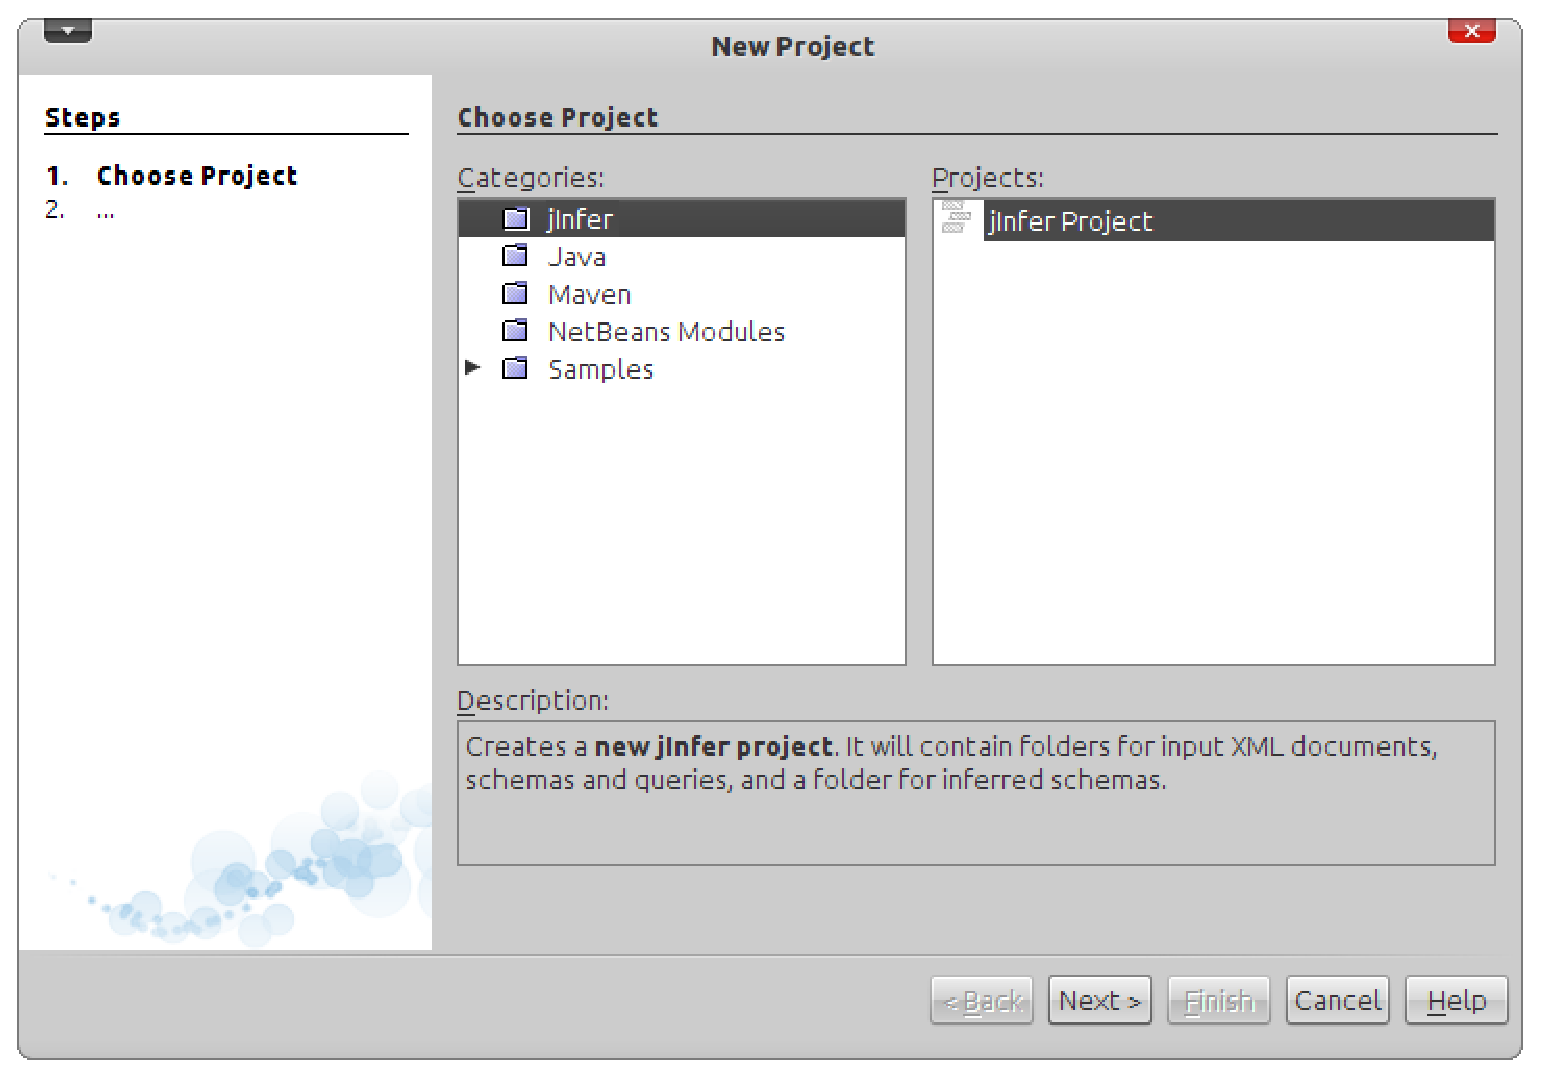
\includegraphics[width=\textwidth]{tutorial_images/new_project}
\end{figure}

Files with XML data, defined functional dependencies and weights assigned to the nodes needs to be added to the newly created project. Files with functional dependencies and weights are xml files with XML Schema shown in Fig. \ref{fdschema} and \ref{weightschema}. These files appears after adding in the \emph{FD} folder of the jInfer project.

\begin{figure}[H]
    \centering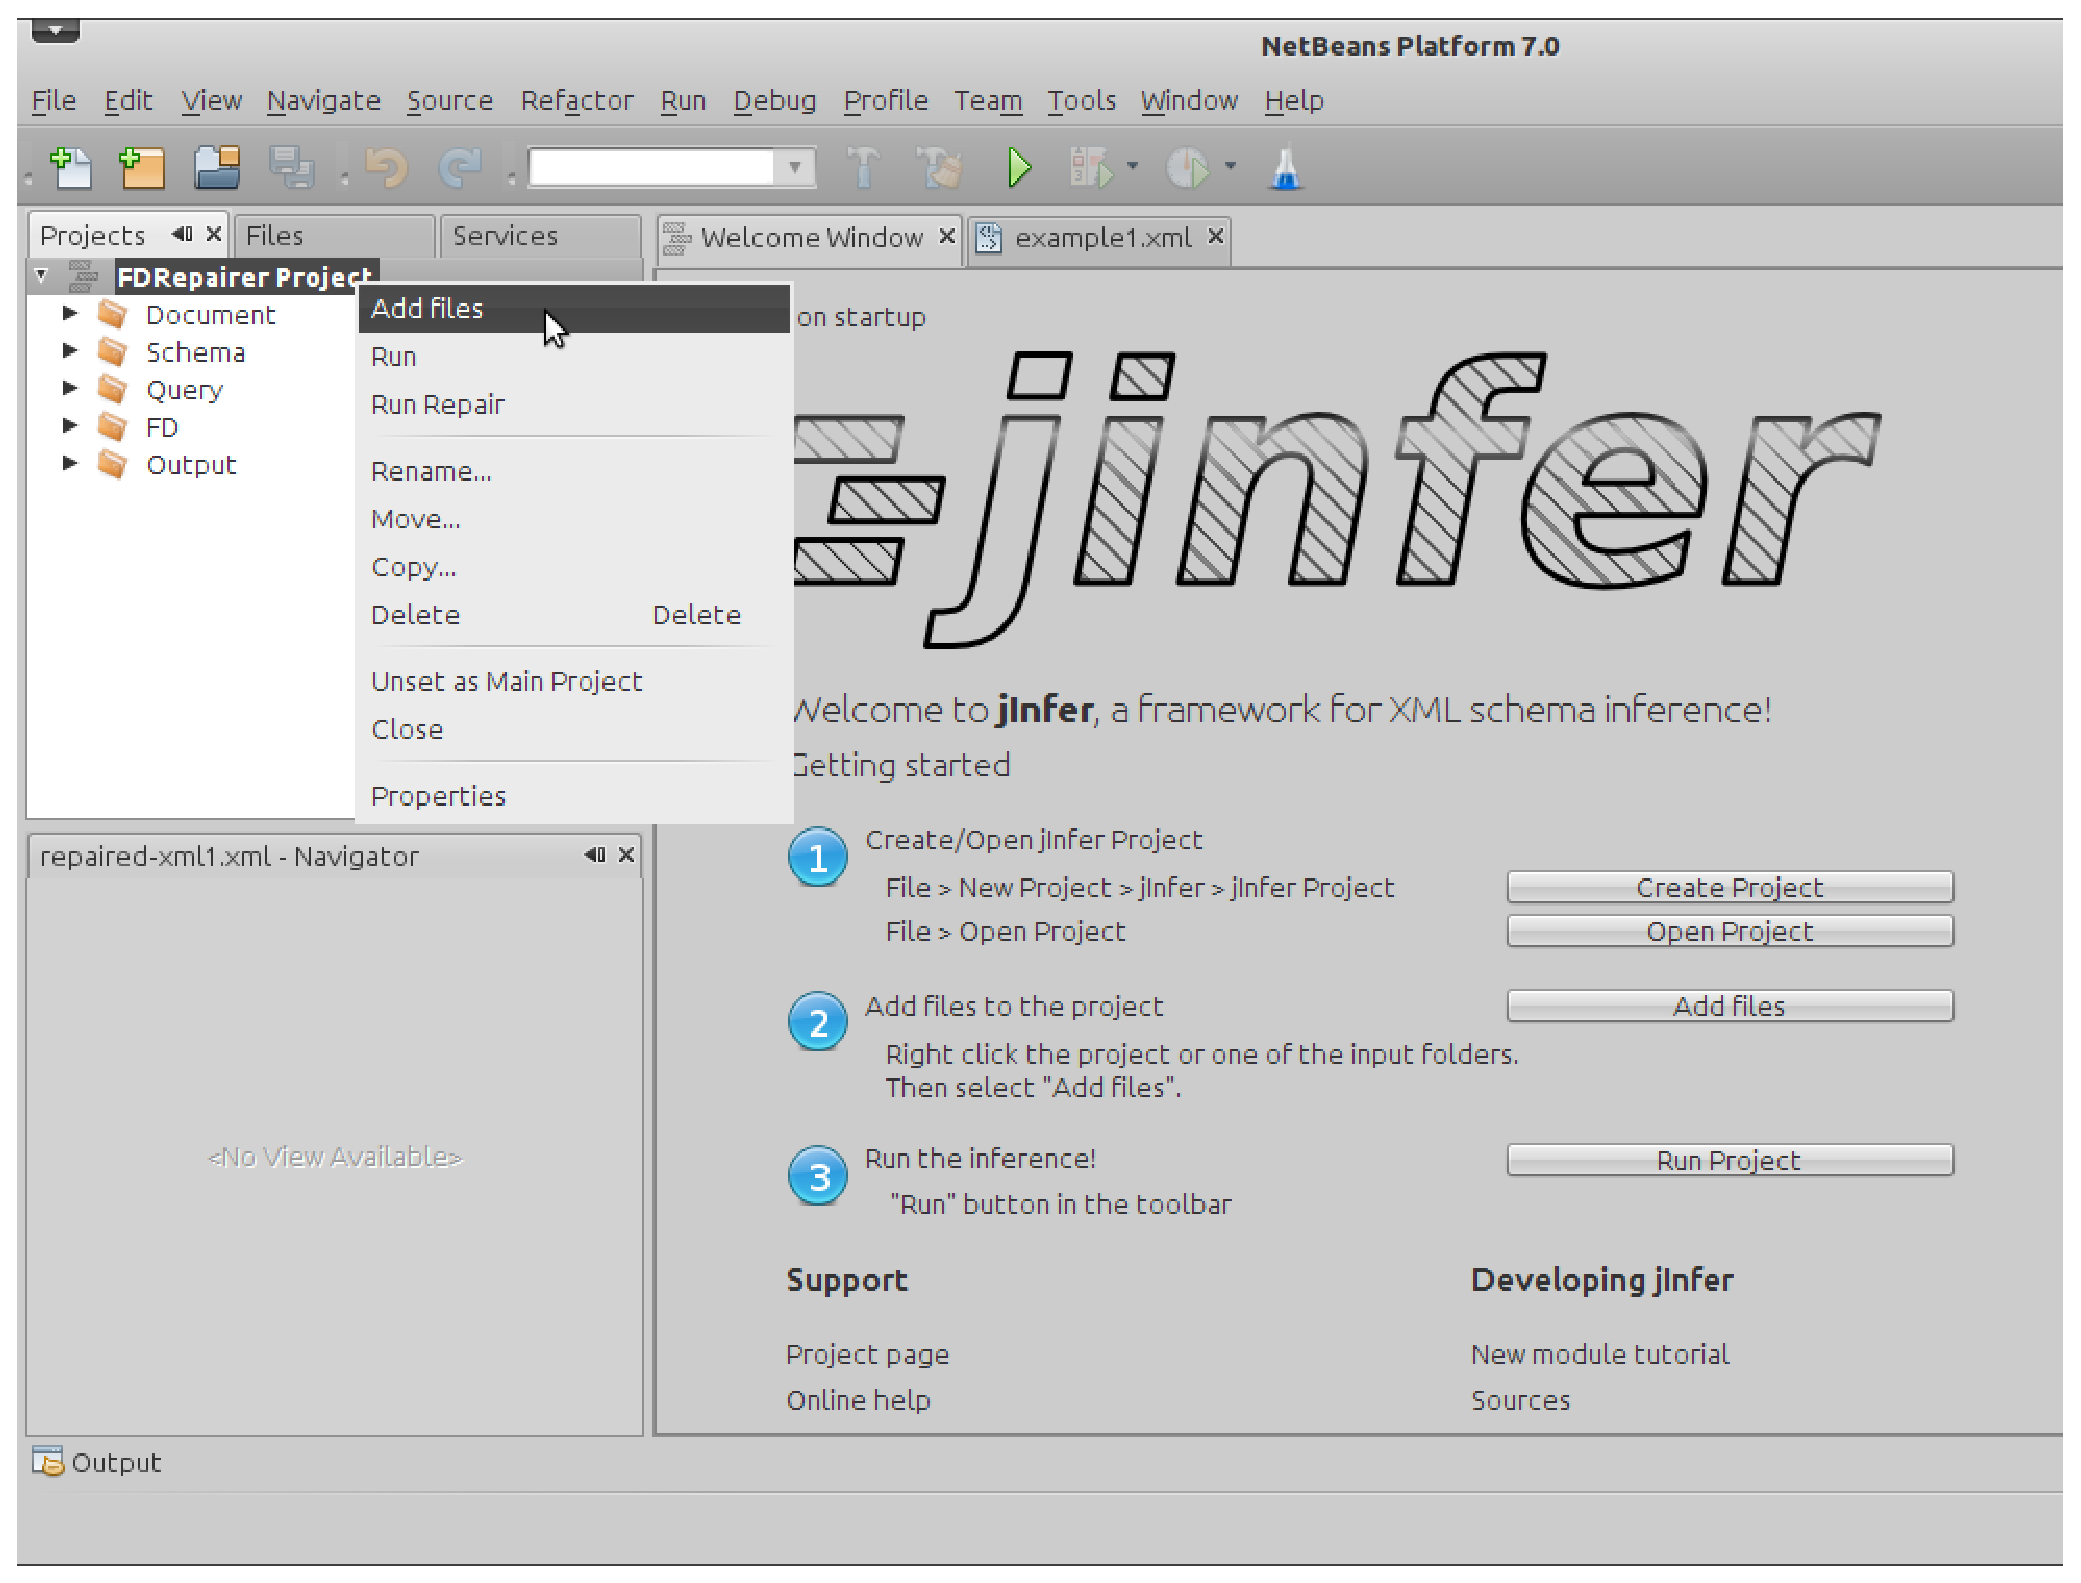
\includegraphics[width=\textwidth]{tutorial_images/add_files}
\end{figure}

The settings of the \texttt{FDRepairer} extension is available in the properties window of the jInfer project accessible through project context menu. In these settings, one could choose between original repairer and repairer proposed in this thesis. For the proposed algorithm is then available to choose between \emph{user interactive} repair picker and \emph{Minimal Repair Picker}. In this place is also possible to set coefficient $k$ and threshold $t$.

\begin{figure}[H]
    \centering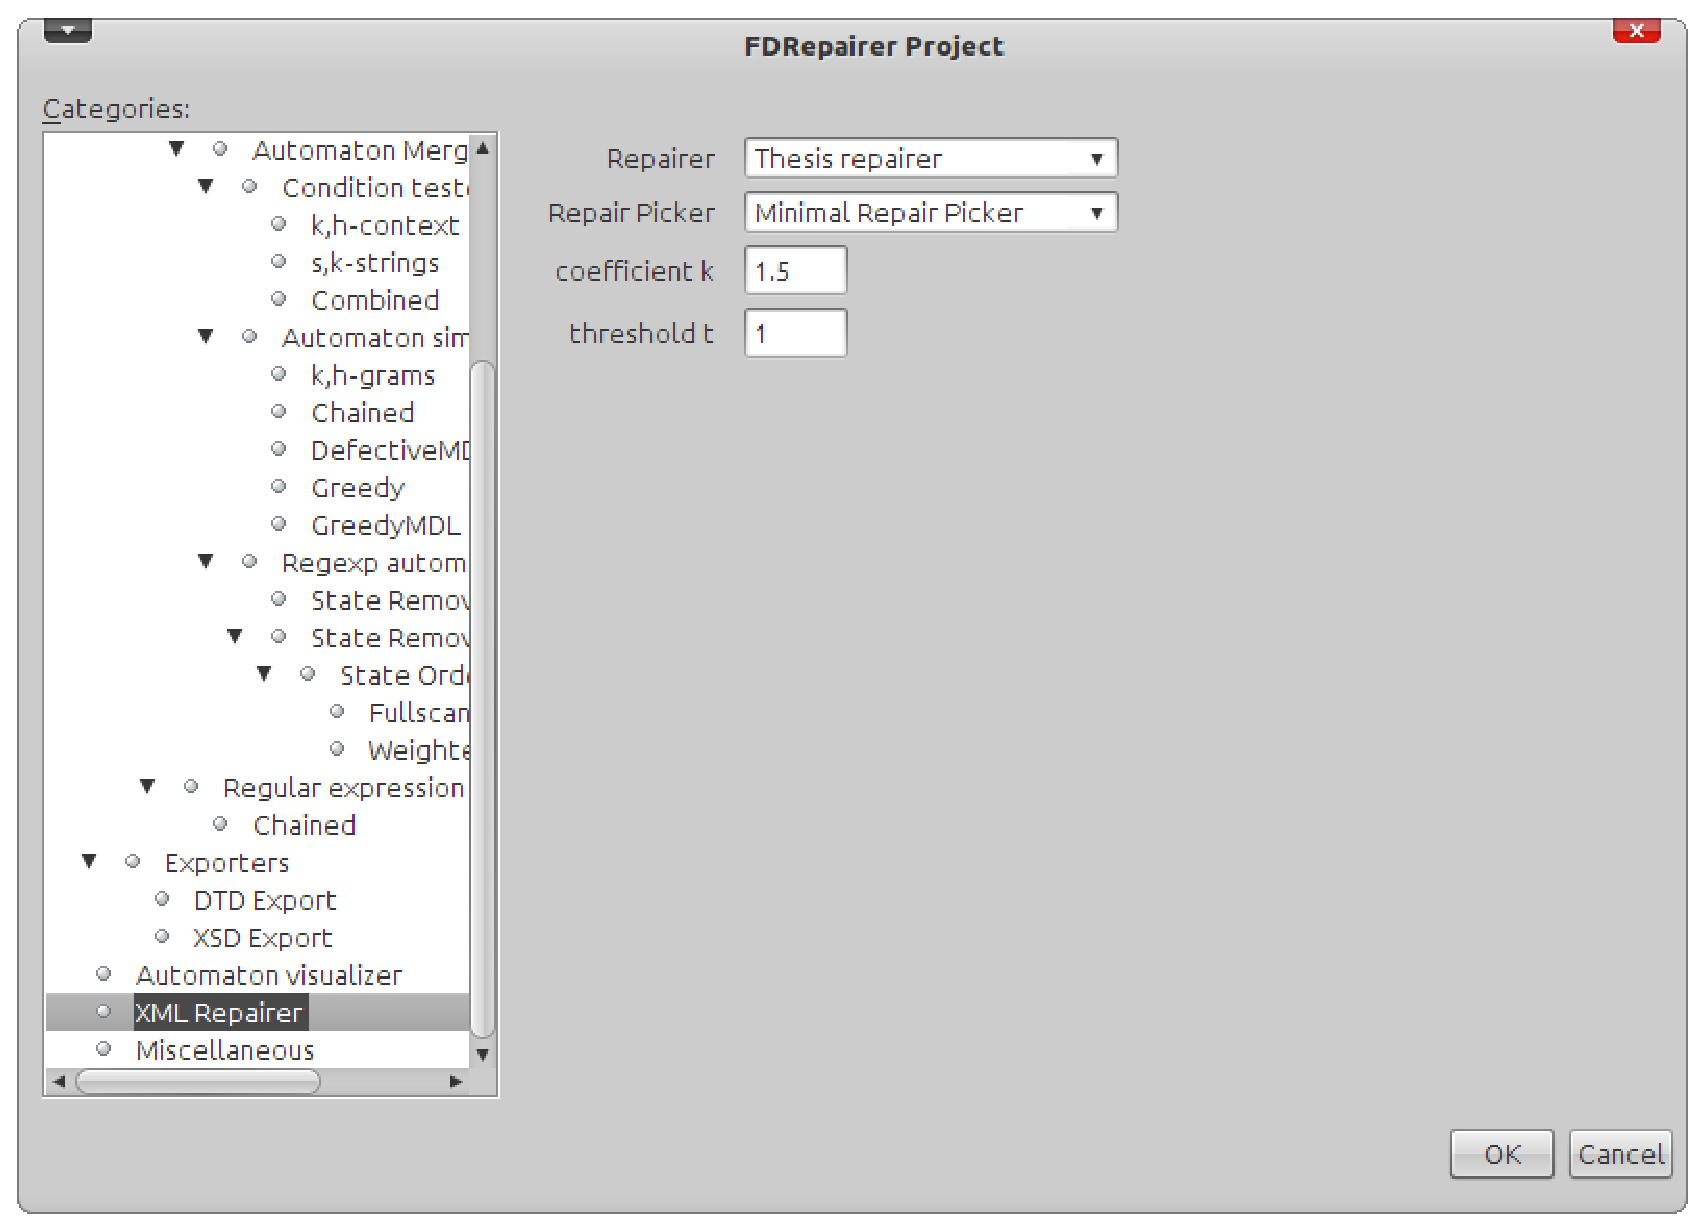
\includegraphics[width=\textwidth]{tutorial_images/project_properties}
\end{figure}

The repair is executed by the \emph{Run Repair} item from the jInfer project context menu:

\begin{figure}[H]
    \centering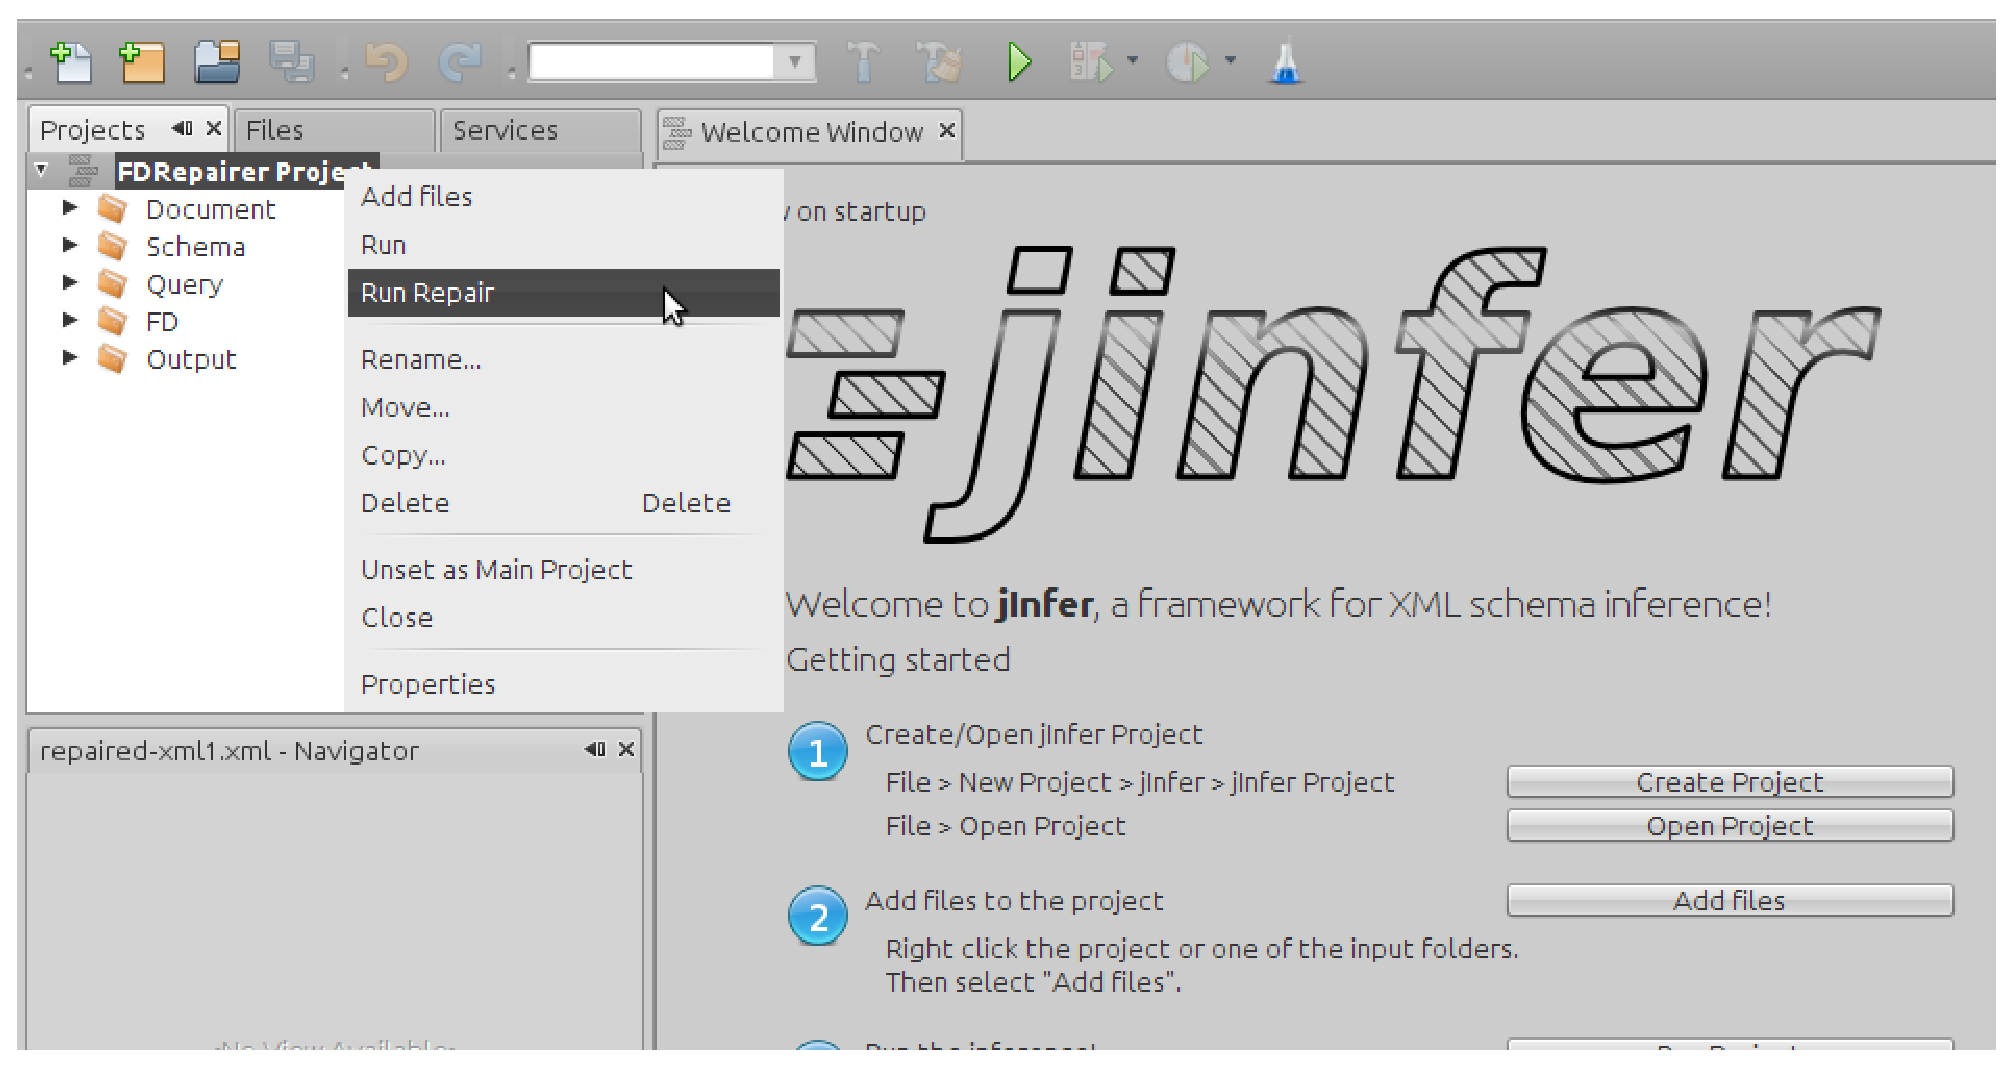
\includegraphics[width=\textwidth]{tutorial_images/run_repair}
\end{figure}

If the \emph{user interactive} repair picker has been selected, \emph{RepairPicker Window} is shown to the user. In this window the user picks repair candidate, which will be applied to the repaired XML.

\begin{figure}[H]
    \centering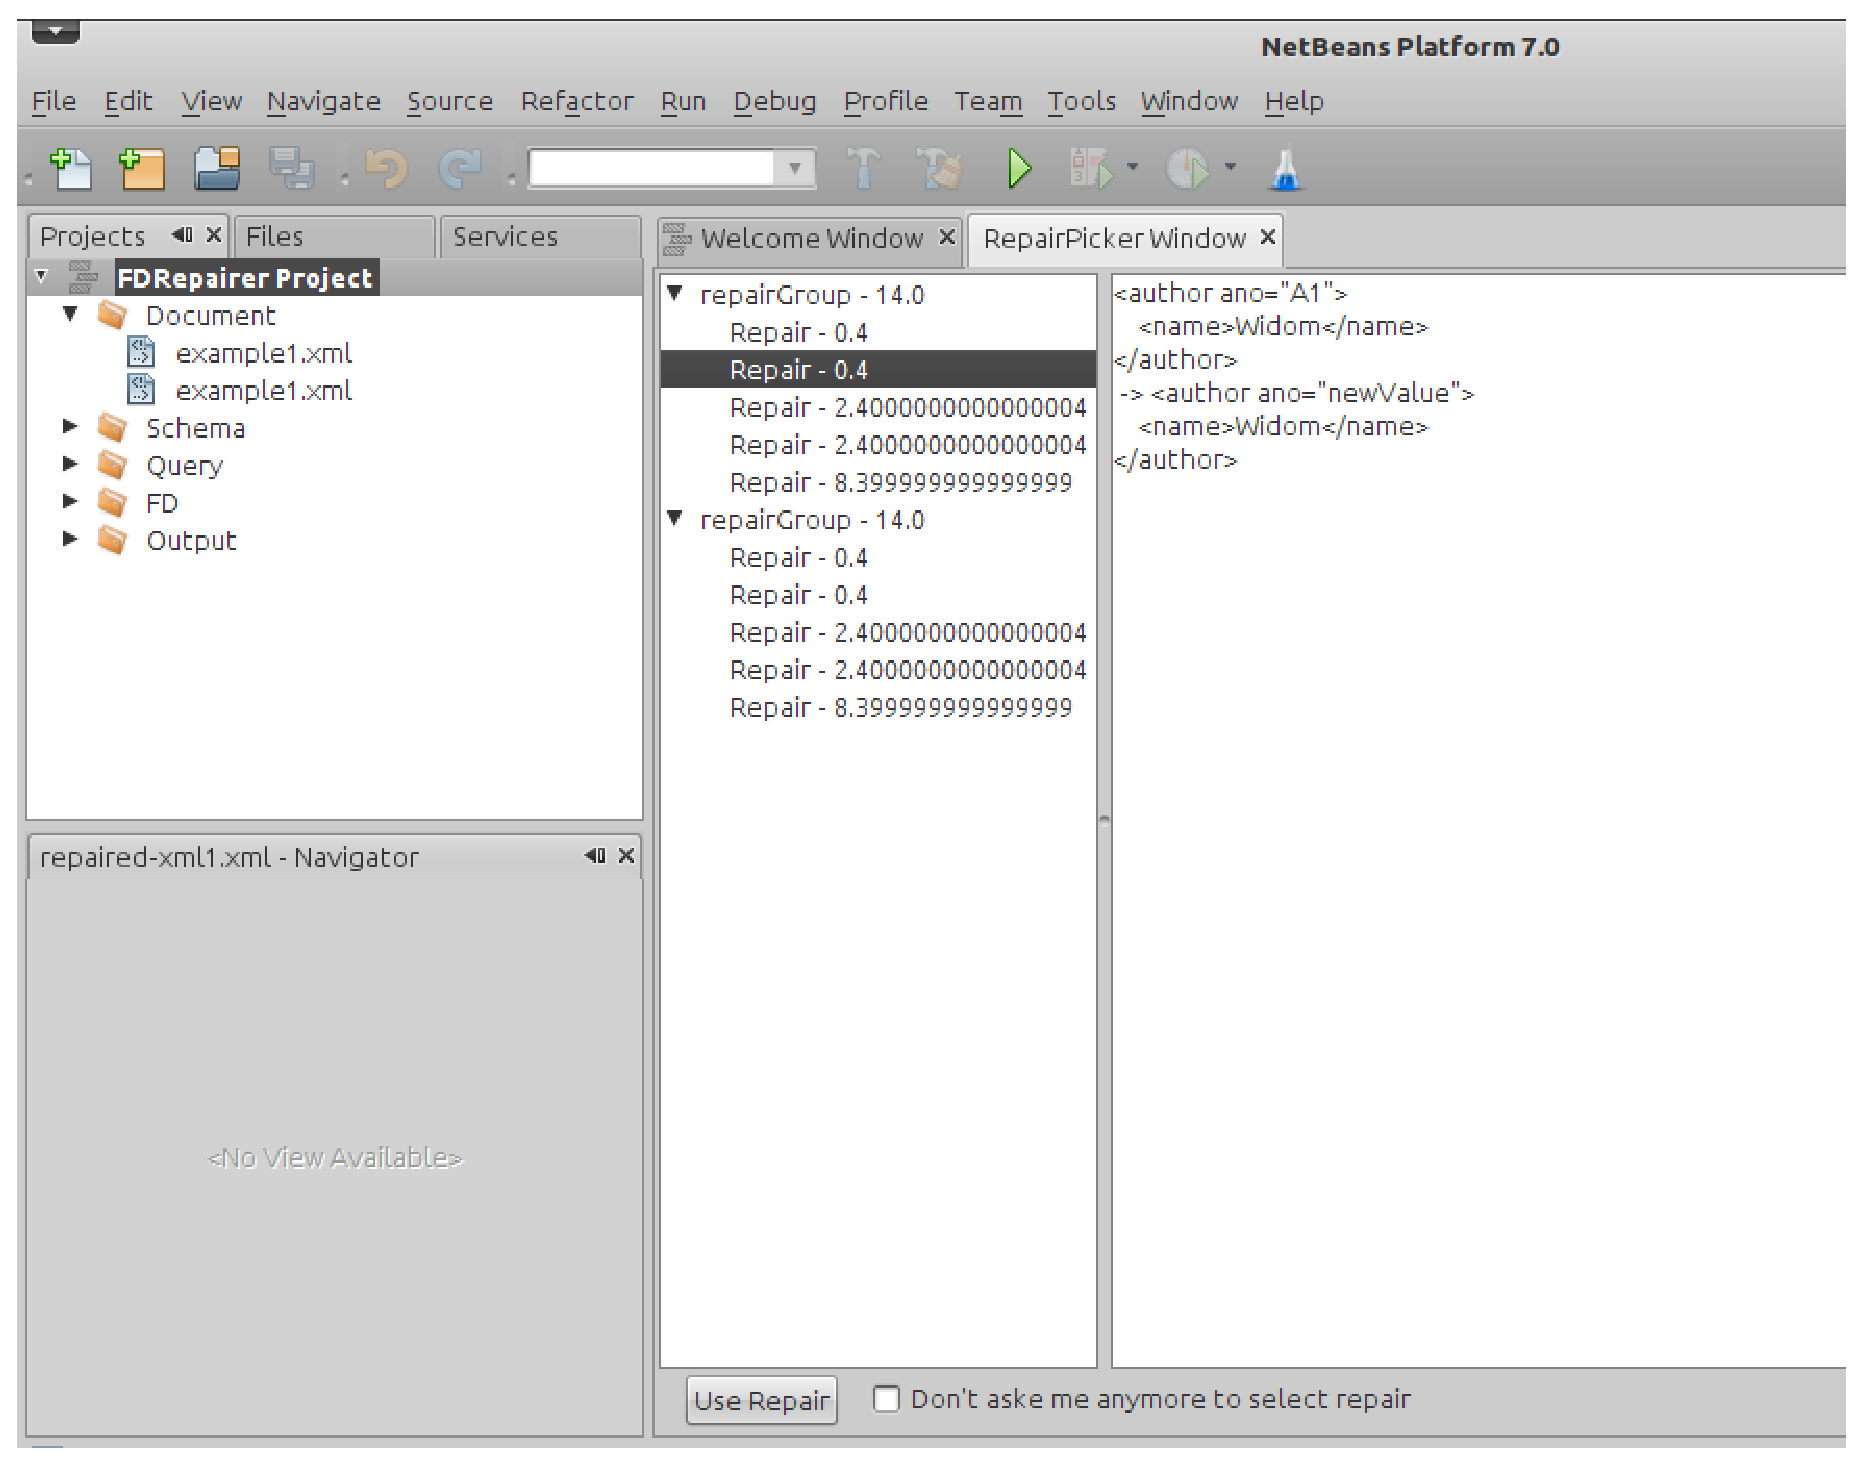
\includegraphics[width=\textwidth]{tutorial_images/user_selection}
\end{figure}

After repairing all the violations, repaired XML document is created in the \emph{Output} subfolder of the jInfer project.
